% !TEX encoding = UTF-8 Unicode 
% !TEX root = praca.tex

\chapter{Oprogramowanie sprzętowe}

\section{Wstęp i wymagania funkcjonalne}
Oprogramowanie makiety sprzętowej stworzono z myślą o następujących wymaganiach funkcjonalnych:

- zapewnienie komunikacji z komputerem PC poprzez interfejs \textit{UART},

- wykrycie podłączenia elektrod i adekwatna zmiana koloru diody \textit{RGB},

- odczyt próbkowanych i kwantyzowanych wartości z przetwornika \textit{ADC},

- wstępne przetwarzanie sygnału przy użyciu filtrów cyfrowych.  

Oprogramowanie sprzętowe napisano głównie w języku \textit{C}, w nieznacznej cześci przy 
pomocy języka \textit{C++}. W implementacji zastosowano również bibliotekę \textit{HAL STM32},
która służyła jako warstwa abstrakcji między sprzętem a oprogramowaniem. Do preprocessingu, 
kompilacji i konsolidacji użyto narzędzi z kolekcji \textit{ARM GNU Embedded Toolchain}. 
Użyto również programów do automatyzacji procesu
budowania oprogramowania takich jak \textit{CMake} oraz \textit{GNU Make}.

\textit{Firmware} był wgrywany do pamięci \textit{EEPROM} 
(\textit{Electrically Erasable Programmable Read-Only Memory}) mikrokontrolera za pomocą
programatora sprzętowego \textit{STLink}.
Programator podłączano poprzez interfejs \textit{USB} do komputera \textit{PC}.
Do przesyłania obrazu pamięci w postaci
pliku binarnego użyto oprogramowania dostarczonego przez producenta: \textit{st-flash} 
\cite{stflash}. Na listingu \ref{listing:stflash} przedsatwiono przykładowe wywołanie wspomnianego
programu, gdzie \textit{ECGMonitor.bin} to binarny obraz programu, natomiast \textit{0x8000000} to
adres (liczba szesnastkowa z prefiksem \textit{0x}) 
pod który zostanie załadowany obraz.

\begin{listing}
\begin{minted}{bash}
st-flash write ECGMonitor.bin 0x8000000
\end{minted}
\caption{Wywołanie programu st-flash do  programu na mikrokontroler}
\label{listing:stflash}
\end{listing}

Po zakończeniu wszystkich kroków procesu budowania \textit{firmwareu} wynikowym plikiem
jest plik ELF (\textit{Executable Linkable Format}) \cite{elfARM}. 
Plik ten zawiera m.in. informacje na temat segmentów programu czy dodatkowych symboli 
do \textit{debugowania}. Format ten jednak nie jest kompatybliny z narzędziem \textit{st-flash}.
Narzędzie to przyjmuje binarny obraz pamięci, który załadowywany jest począwszy od wskazanego
w linii poleceń adresu. Do wygenerowania obrazu pamięci z pliku \textit{ELF}, zastosowano program 
\textit{arm-none-eabi-objcopy} z kolekcji \textit{ARM GNU Embedded Toolchain}.

\section{Akwizycja sygnału}

W oprogramowaniu sprzętowym użyto wbudowanego w mikrokontroler kontrolera \textit{DMA}, który połączony jest
osobną od rdzenia magistralą z innymi układami peryferyjnymi i pamięcią. Umożliwia to niemal niezależne
transfery danych między przetwornikiem analogowo-cyfrowym a pamięcią.
W celu osiągnięcia precyzyjnej częstotliwości próbkowania $f_s = 360 Hz$ wykorzystano wbudowany układ licznika
o rozdzielczości 16 bitów, który skonfigurowano by zliczał w naturalnym kodzie binarnym modulo 512 z częstotliwością 
$f_c \approx 184,3 kHz$ i generował przerwanie przy każdym przepełnieniu. W kontrolerze przerwań skonfigurowano ten 
typ przerwania w taki sposób aby każdorazowo wywoływało konwersję przetwornika analogowo-cyfrowego, a przewanie
końca konwersji wywoływało transfer \textit{DMA} z przetwornika do bufora kołowego w pamięci mikrokontrolera.
W rutynie przerwania sygnalizującego koniec transferu \textit{DMA} umieszczono fragment kodu przedstawiony na listingu
\ref{listing:dmairq}.

\begin{listing}
\begin{minted}{c}
__disable_irq();
adc_buffer_last_index = (adc_buffer_last_index + 1) % ADC_BUF_LEN;
__enable_irq();
\end{minted} 
\caption{Fragment rutyny przerwania dla zakończenia transferu \textit{DMA} z przetwornika \textit{ADC} do pamięci}
\label{listing:dmairq}
\end{listing}

Funkcje \textit{\_\_disable\_irq} i \textit{\_\_enable\_irq} odpowiadają kolejno za tymczasowe wyłączanie obsługi przerwań 
i jej ponowne włączenie.
Zmienna \textit{adc\_buffer\_last\_index} przechowuje indeks na którym zostanie zapisana kolejna próbka w buforze kołowym, będącym
tablicą o długości \textit{ADC\_BUF\_LEN} i rozmiarze elemtów równym dwóm bajtom (rozmiar każdej z próbek). Wartość
indeksu jest inkrementowana, dzięki operacji modulo nie przekracza zakresu tablicy i wraca na jej początek po dotarciu do końca.
Wspomniane \textit{\_\_disable\_irq} i \textit{\_\_enable\_irq} funkcje zastosowanu w tym przypadku aby zapewnić 
atomowość operacji inkrementacji indeksu w buforze kołowym, innymi słowy by nie dopuścić innych przerwań do 
potencjalnego opóźnienia tak krytycznej dla działania sprzętu operacji.


Odczyt danych z bufora kołowego odbywa się przy założeniu że rdzeń odczytuje próbki z bufora kołowego na tyle szybko,
że nigdy nie dojdzie do sytuacji gdy dane jeszcze nieodczytane zostaną nadpisane nowymi. Do śledzenia indeksu odczytu
zdefiniowano zmienną globalną \textit{adc\_buffer\_curr\_index}, na rysunku \ref{fig:rbuffer} przedstawiono bufor
kołowy w skrajnym przypadku gdzie jest on zapełniony i w przypadku nieodczytania danych dostatecznie szybko, dane zostaną utracone.
Podobnie jak w przypadku \textit{adc\_buffer\_last\_index}, wspomniana zmienna globalna jest inkrementowana przy każdym odczycie
wraz z wykonaniem analogicznej operacji modulo.

\begin{figure}[h!]
    \centering 
    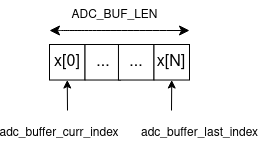
\includegraphics[scale=0.7]{pl/media/rbuffer.png}
    \caption{Rysunek poglądowy bufora kołowego zwierającego próbki sygnału}
    \label{fig:rbuffer}
\end{figure}

\newpage
\section{Implementacja filtrów FIR}

Obecność jednostki zmiennoprzecinkowej \textit{FPU} (\textit{Floating-point Unit}) w rdzeniu \textit{ARM Cortex M4} 
mikrokontrolera umożliwia szybkie operacje na liczbach zmiennoprzecinkowych bez konieczności implementacji tych operacji 
w oprogramowaniu. Z racji na to zdecydowano, że współczynniki filtrów \textit{FIR} przechowywane będą w pamięci 
mikrokontrolera jako liczby zmiennoprzecinkowe pojedynczej precyzji w standardzie \textit{IEEE-754}. Użycie typu
zmiennoprzecinkowego umożliwia łatwe przeniesienie współczynników wyliczonych podczas projektowania filtru na mikrokontroler.

\begin{listing}
\begin{minted}{c}
#include <inttypes.h>

typedef float fp32_t;

struct fir_t
{
  const fp32_t* coeffs;
  uint32_t coeffs_len;
  volatile uint16_t* buf;
  uint32_t buf_len; 
};
\end{minted} 
\caption{Struktura fir\_t}
\label{listing:firt}
\end{listing}

Na listingu \ref{listing:firt} przedstawiono strukturę przekazywaną potem do funkcji realizującej dyskretny splot sygnału z
współczynnikami filtru. Pole \textit{coeffs} jest wskaźnikiem (adresem) na stałą tablicę współczynników zapisaną w pamięci
mikrokontrolera ustawianą podczas kompilacji oprogramowania, zawartą w wynikowym w pliku wykonywalnym wgrywanym do pamięci 
\textit{EEPROM} mikrokontrolera. Pole \textit{buf} jest wskaźnikiem do bufora kołowego zawierającego próbkowany sygnał.
Natomiast pola \textit{coeffs\_len} oraz \textit{buf\_len} oznaczają odpowiednio długości tablic: 
współczynników oraz bufora kołowego.
Pole \textit{buf} wymaga dopisanego słowa kluczowego \textit{volatile} ze względu na naturę zapisów do wspomnianego bufora: poprzez
przerwania i transfery DMA. 


W wypadku buforów modyfikowanych przez rutyny przerwań lub inne mechanizmy sprzętowe 
pojawia się następujący problem: kompilator języka \textit{C} nie posiadając kontekstu i informacji na temat architektury maszyny
na jakiej program będzie wykonywany, traktuje rutyny przerwań jako funkcje które nigdy nie zostają wywołane. Zatem jeżeli do zapisu
danych do bufora nie dochodzi w innych częściach programu, to kompilator może zoptymalizować wszystkie odczyty danych 
z bufora poprzez wstawienie we wspomniane miejsca instrukcji odczytania zera przechowanego np. w rejestrze procesora, 
zamiast kosztownego odczytu z pamięci. Słowo kluczowe \textit{volatile} jest sugestią dla kompilatora, aby ten nie przeprowadzał
optymalizacji w przypadku danego fragmentu pamięci, adresu, zmiennej lub funkcji.


Działanie filtru FIR implementuje funkcja \textit{fir\_convolve} przedstawiona na listingu \ref{listing:firconv}. 
Funkcja ta realizuje operację splotu dyskretnego próbek sygnału ze współczynnikami flitru:

$$
(f * g)[n] = \sum_{k=-\infty}^{\infty} f[k]g[n-k]
$$

\begin{listing}
\begin{minted}{c}
fp32_t fir_convolve(struct fir_t* fir, uint32_t pos)
{ 
    uint32_t buf_idx = pos; 
    fp32_t result = 0.0f;
  
    for(uint32_t c_idx = fir->coeffs_len; c_idx != 0 ; --c_idx) { 
        result += (fir->buf[buf_idx] * fir->coeffs[c_idx - 1]);
        buf_idx = (buf_idx + 1) % fir->buf_len;
    }     
  
    return result;
} 
\end{minted} 
\caption{Funkcja realizaująca splot dyskretny próbek sygnału ze współczynnikami filtru FIR}
\label{listing:firconv}
\end{listing}

\newpage

\section{Wykrywanie podłączonych elektrod}

Układ \textit{AD8232} udostępnia dwa wyprowadzenia do wykrywania odłączonych elektrod oznaczone \textit{LOD-} i \textit{LOD+}.
W wypadku gdy jedna lub więcej elektrod jest niepodłączona to conajmniej jedno z wyprowadzeń jest w stanie wysokim 
(logiczna 1).
Wykrywanie podłączonych elektrod zrealizowano dzięki możliwości generowania przerwań zewnętrznych poprzez wykrycie zmiany
stanu wyprowadzenia mikrokontrolera. Wyprowadzenia (połączone z \textit{LOD-} i \textit{LOD+}) w odpowiednich portach 
wejścia/wyjścia ogólnego przeznaczenia (\textit{GPIO}, \textit{General Purpose Input/Output})
skonfigurowano tak, aby generowały przerwanie przy wykryciu zbocza opadającego lub narastającego. 
Dla obu tych przerwań zewnętrznych w wektorze przerwań ustawiono ten sam adres rutyny obsługującej przerwanie.

\begin{listing}
\begin{minted}{c}
void EXTI9_5_IRQHandler(void)
{
  if( (HAL_GPIO_ReadPin(LOD_N_GPIO_Port, LOD_N_Pin) == 0) &&
      (HAL_GPIO_ReadPin(LOD_P_GPIO_Port, LOD_P_Pin) == 0) )
  {
    __disable_irq();
    HAL_GPIO_WritePin(LED_RED_GPIO_Port, LED_RED_Pin, 1);
    HAL_GPIO_WritePin(LED_GREEN_GPIO_Port, LED_GREEN_Pin, 0);
    leads_off = false;
    __enable_irq();
  }
  else
  {
    __disable_irq();
    HAL_GPIO_WritePin(LED_RED_GPIO_Port, LED_RED_Pin, 0);
    HAL_GPIO_WritePin(LED_GREEN_GPIO_Port, LED_GREEN_Pin, 1);
    leads_off = true;
    __enable_irq();
  }
\end{minted} 
\caption{Fragment rutyny obsługi przerwania zewnętrznego 
          realizujący wykrywanie odłączonych elektrod}
\label{listing:leadsoff}
\end{listing}

Fragment kodu wspomnianej procedury osbługi przerwania przedstawiono na listingu \ref{listing:leadsoff}.
Funkcje z przedrostkiem \textit{HAL\_GPIO\_} są funkcjami biblioteki \textit{HAL STM32}. Funkcja
\textit{ReadPin} odczytuje wartość logiczną danego wejścia w danym porcie \textit{GPIO}, natomiast
\textit{WritePin} ustawia zadaną wartość na wyjściu danego wyprowadzenia. W programie użyto zmiennej globalnej
\textit{leads\_off}, która gdy jest równa prawdzie, oznacza że elektrody nie są podpięte prawidłowo do ciała pacjenta.
W przypadku wykrycia odłączenia kolor diody \textit{RGB} na płytce z mikrokontrolerem ustawiany jest na czerwony, w
przeciwnym wypadku na kolor zielony (konkretne kolory aktywowane są wartością \textit{0}).

\section{Komunikacja z użyciem interfejsu UART}

Dla prostoty komunikacji urządzenia z komputerem PC zastosowano komunikację jednokierunkową,
urządzenie wysyła dane poprzez interfejs zawsze kiedy wykryje podpięte elektrody a w buforze kołowym znajdują 
się nowe próbki do odczytu.

